\chapter{ワークA：センサ回路設計}

\section{はじめに}
%% ワークAを理解した上で，目的として要約する
%%
%% （例文）
%% 本課題では～を目的とし，～の実験を行った．
%% 実験を通じて～の結果を得た．
%% それらの結果より，～であることを明らかにする．

本課題では，フォトリフレクタを用いて脈拍のような微弱な信号を検出し，
後の処理に適した信号に増幅し，ノイズ除去を行う回路の設計と実装を通じて，アナログ回路の基本を学ぶことを目的とする．
実験では，オペアンプを用いたバンドパスフィルタ付き二段反転増幅回路を設計，実装した．
実験を通じて，設計した回路が信号を増幅，不要な周波数成分を除去できることを確認し，実際の脈拍を検出し増幅した観測結果を得た．
それらの結果より，微弱なセンサ信号からノイズを除去し，必要な信号のみを増幅するフィルタ増幅回路の有効性を明らかにする．




\section{方法及び手順} 
%% ワークAで設計・実装するものを理解した上で，方法や手順に落とし込んだ
%% 形で，客観的に記述する．報告書の基準は，この報告書の記述だけで，第
%% 三者が追試をし，同様の結果を得ることできることである．必要に応じて，
%% 図，表，式を用いて，曖昧な箇所や誤解を生じにくい説明が求められる．



\subsection{原理}
本実験で用いる脈拍測定の原理と，主要な電子部品の動作原理を以下に示す．


\subsubsection{脈拍測定の原理}
本実験では，光電容積脈波法の中でも，センサを身体の表面に当てることで計測が可能な反射型の方式を用いた．
これは，指先に赤外線を照射し，心臓の拍動に伴う毛細血管の血流量の変化に応じて変化する反射光の強度を測定することで脈波を得る手法である\cite{安藤譲二1990光電式脈波計測の応用}．
血流量が多くなると光の吸収量が増加して反射光は減少し，逆に血流量が少なくなると光の吸収量が減少して反射光は増加する\cite{hertzman1938blood}．
この反射光の周期的変化を電気信号として捉えることで，脈拍を測定する．


\subsubsection{フォトリフレクタ(LBR-127HLD)}
本実験で用いるフォトリフレクタ(LBR-127HLD)は，赤外線発光ダイオードとフォトトランジスタが一つのパッケージに収められた反射型光センサである\cite{LBR-127HLD}．
LEDから照射された赤外線が指先で反射し，その光をフォトトランジスタが受光する．
フォトトランジスタは，受光した光の強度に応じてコレクタ-エミッタ間に流れる電流が変化する素子であり\cite{workA_フォトトランジスタ}，
この電流の変化を抵抗によって電圧の変化に変換することで，脈波信号を出力する．


\subsubsection{オペアンプ(LM358N)を用いた信号処理}
\paragraph{反転増幅回路}
フォトリフレクタから出力される信号は微弱であるため，オペアンプを用いた反転増幅回路によって後段の処理に適した電圧レベルまで増幅する．
反転増幅回路の増幅率 $A$ は，入力抵抗 $R_s$ と帰還抵抗 $R_f$ の比によって決まり，以下の式で表される\cite{workA_オペアンプ}．
\begin{equation}
  A = - \frac{R_f}{R_s} \label{eq:A}
\end{equation}

\paragraph{バンドパスフィルタ}
脈波の周波数はおおよそ0.5Hzから2Hz程度であるため，測定時には体動による低周波の揺らぎや，商用電源などに起因する高周波ノイズが問題となる\cite{workA_脈拍周波数}．
これらの不要な信号成分を除去するため，ハイパスフィルタとローパスフィルタを組み合わせたバンドパスフィルタを実装する．
本回路では，オペアンプを用いたアクティブフィルタを構成し，入力抵抗$R_s$と直列に接続されたコンデンサを$C_s$，帰還抵抗$R_f$と並列に接続されたコンデンサを$C_f$とすると，
下限周波数 $f_L$ と上限周波数 $f_U$ は以下の式によって決定される\cite{workA_バンドパスフィルタ}．
\begin{equation}
  f_L = \frac{1}{2\pi C_s R_s} \label{eq:f_L}
\end{equation}
\begin{equation}
  f_U = \frac{1}{2\pi C_f R_f} \label{eq:f_U}
\end{equation}




\subsection{回路設計と使用部品}
本実験で実装した回路の設計計算と，それに基づき選定した使用部品について述べる．
まず信号を増幅・フィルタリングする後段回路の設計について述べ，次に入力となる脈拍検出部の設計について述べる．


\subsubsection{バンドパスフィルタ付き二段反転増幅回路の設計}
センサから得られる微弱な信号を処理するため，バンドパスフィルタ付き二段反転増幅回路を設計した．設計仕様は以下の通りである．

\paragraph{増幅率}
全体で約+91.8倍の増幅率を得るため，一段目を-30.3倍，二段目を-3.03倍に設定した．式(\ref{eq:A})に基づき，各抵抗値を式(\ref{eq:A_1})，式(\ref{eq:A_2})ように選定した．
\begin{equation}
  A_1 = -\frac{R_2}{R_5} = -\frac{1\text{M}\Omega}{33\text{k}\Omega} \approx -30.3 \label{eq:A_1}
\end{equation}
\begin{equation}
  A_2 = -\frac{R_1}{R_6} = -\frac{100\text{k}\Omega}{33\text{k}\Omega} \approx -3.03 \label{eq:A_2}
\end{equation}
この計算に基づき，$R_1=100\text{k}\Omega$, $R_2=1\text{M}\Omega$, $R_5=R_6=33\text{k}\Omega$を選定した．

\paragraph{周波数帯域}
下限周波数 $f_L \approx 0.48$ Hz，上限周波数 $f_U \approx 16$ Hzのバンドパス特性を得るよう，式(\ref{eq:f_L})および式(\ref{eq:f_U})に基づきコンデンサを選定した．
\begin{itemize}
  \item 下限周波数($f_L$): 主に$C_3$，$R_5$と$C_4$，$R_6$のハイパスフィルタで決定される．
  $C_3$，$C_4$を$10\mu\text{F}$とすると，式(\ref{eq:low_1})および式(\ref{eq:low_2})となり，回路全体の下限周波数は約0.48Hzとなる．
  \begin{equation}
    f_{L1} = \frac{1}{2\pi R_5 C_3} = \frac{1}{2\pi \times 33\text{k}\Omega \times 10\mu\text{F}} \approx 0.48 \text{Hz} \label{eq:low_1}
  \end{equation}
  \begin{equation}
    f_{L2} = \frac{1}{2\pi R_6 C_4} = \frac{1}{2\pi \times 33\text{k}\Omega \times 10\mu\text{F}} \approx 0.48 \text{Hz} \label{eq:low_2}
  \end{equation}
  したがって，$C_3=C_4=10\mu\text{F}$を選定した．
  \item 上限周波数($f_U$): 主に$R_2$，$C_2$と$R_1$，$C_1$のローパスフィルタで決定される．
  $C_2$を$0.010\mu\text{F}$, $C_1$を$0.10\mu\text{F}$とすると，式(\ref{eq:high_1})および式(\ref{eq:high_2})となり，回路全体の上限周波数は約16Hzとなる．
  \begin{equation}
    f_{U1} = \frac{1}{2\pi R_2 C_2} = \frac{1}{2\pi \times 1\text{M}\Omega \times 0.010\mu\text{F}} \approx 16 \text{Hz} \label{eq:high_1}
  \end{equation}
  \begin{equation}
    f_{U2} = \frac{1}{2\pi R_1 C_1} = \frac{1}{2\pi \times 100\text{k}\Omega \times 0.10\mu\text{F}} \approx 16 \text{Hz} \label{eq:high_2}
  \end{equation}
  したがって，$C_2=0.010\mu\text{F}$，$C_1=0.10\mu\text{F}$を選定した．
\end{itemize}
    
\paragraph{バイアス回路}
本回路は+5Vの単電源で動作させるため，抵抗分圧によるバイアス回路を設けた．
抵抗$R_8=R_{10}=100\text{k}\Omega$と$R_7=R_9=33\text{k}\Omega$を用いて基準電圧を生成し，これを各オペアンプの非反転入力端子(+)に加えている．


\subsubsection{脈拍検出回路の設計}
増幅・フィルタ回路に入力するための信号を生成するセンサ部として，脈拍検出回路を設計した．設計仕様は以下の通りである．

\paragraph{赤外LEDの電流制限抵抗($R_3$)}
赤外LEDを適切な光量で発光させるため，電流制限抵抗 $R_3$ の値を決定した．
仕様の標準値である順方向電流 $I_F$ を20mA，その際の順方向電圧 $V_F$ を1.5Vとすると\cite{LBR-127HLD}，5V電源において必要な抵抗値は式(\ref{eq:led})より算出できる．
\begin{equation}
  R_3 = \frac{V_{CC} - V_F}{I_F} = \frac{5\text{V} - 1.5\text{V}}{20\text{mA}} = 175 \Omega \label{eq:led}
\end{equation}
本実験では，計算値の2倍弱の抵抗値として$330 \Omega$を選定した．

\paragraph{フォトトランジスタの負荷抵抗($R_4$)}
フォトトランジスタの負荷抵抗($R_4$): フォトトランジスタが受光した光の強度変化を電圧の変化に変換するため，負荷抵抗 $R_4$ の値を決定した．
フォトトランジスタに光が照射され飽和した際のコレクタ-エミッタ間飽和電圧 $V_{CE(sat)}$ を0.4V，その際のコレクタ電流 $I_C$ を2mAとすると\cite{LBR-127HLD}，
5V電源において必要な抵抗値は，式(\ref{eq:ft})より算出できる．
\begin{equation}
  R_4 = \frac{V_{CC} - V_{CE(sat)}}{I_C} = \frac{5\text{V} - 0.4\text{V}}{2\text{mA}} = 2300 \Omega \label{eq:ft}
\end{equation}
%本実験で使用可能な抵抗器のうち，計算値の2倍($1700\Omega$)に近いものは$330\Omega$と$3.3k\Omega$であった．
%ここで，$R_4$ の値は，脈波による微弱な電流変化を電圧変化に変換する感度を決定する要素であり，抵抗値が大きいほど感度は向上する．
%計算値より低い$330\Omega$では感度が不足する可能性があるため，より高い感度が得られる$3.3k \Omega$を選定した．
%これにより，脈波の微細な変化をより大きな電圧振幅として後段回路に伝えることが期待できる．
本実験では，計算値の2倍弱の抵抗値として$3.3k \Omega$を選定した．


\subsubsection{使用部品一覧}
以上の設計計算に基づき選定した部品の一覧を表\ref{tab:parts_list}にまとめる．
\begin{table}[H]
  \caption{部品表}
  \centering
  \begin{tabular}{|l|c|l|l|}
    \hline
    部品名 & 数量 & 仕様 & 素子変数 \\
    \hline \hline
    炭素皮膜抵抗 & 1 & $330 \Omega$ & $R_3$ \\
    \hline
    炭素皮膜抵抗 & 1 & $3.3k \Omega$ & $R_4$ \\
    \hline
    炭素皮膜抵抗 & 4 & $33k \Omega$ & $R_5, R_6, R_7, R_9$ \\
    \hline
    炭素皮膜抵抗 & 2 & $1M \Omega$ & $R_2, R_{11}$ \\
    \hline
    炭素皮膜抵抗 & 3 & $100k \Omega$ & $R_1, R_8, R_{10}$ \\
    \hline
    積層セラミックコンデンサ & 2 & $10 \mu F$ & $C_3, C_4$ \\
    \hline
    積層セラミックコンデンサ & 1 & $0.010 \mu F$ & $C_2$ \\
    \hline
    積層セラミックコンデンサ & 1 & $0.10 \mu F$ & $C_1$ \\
    \hline
    オペアンプ & 1 & LM358N & - \\
    \hline
    フォトリフレクタ & 1 & LBR-127HLD & - \\
    \hline
    オシロスコープ & 1 & Tektronix TBS1000C & - \\
    \hline
    波形出力デバイス & 1 & ATOM Lite & - \\
    \hline
  \end{tabular}
  \label{tab:parts_list}
\end{table}

\newpage

\subsubsection{回路図}
表\ref{tab:parts_list}から作成した回路図を図\ref{fig:1_fig}，図\ref{fig:2_fig}に示す．
図\ref{fig:1_fig}はワークA-1，図\ref{fig:2_fig}はワークA-2の回路図である．
\begin{figure}[H]
  \centering
  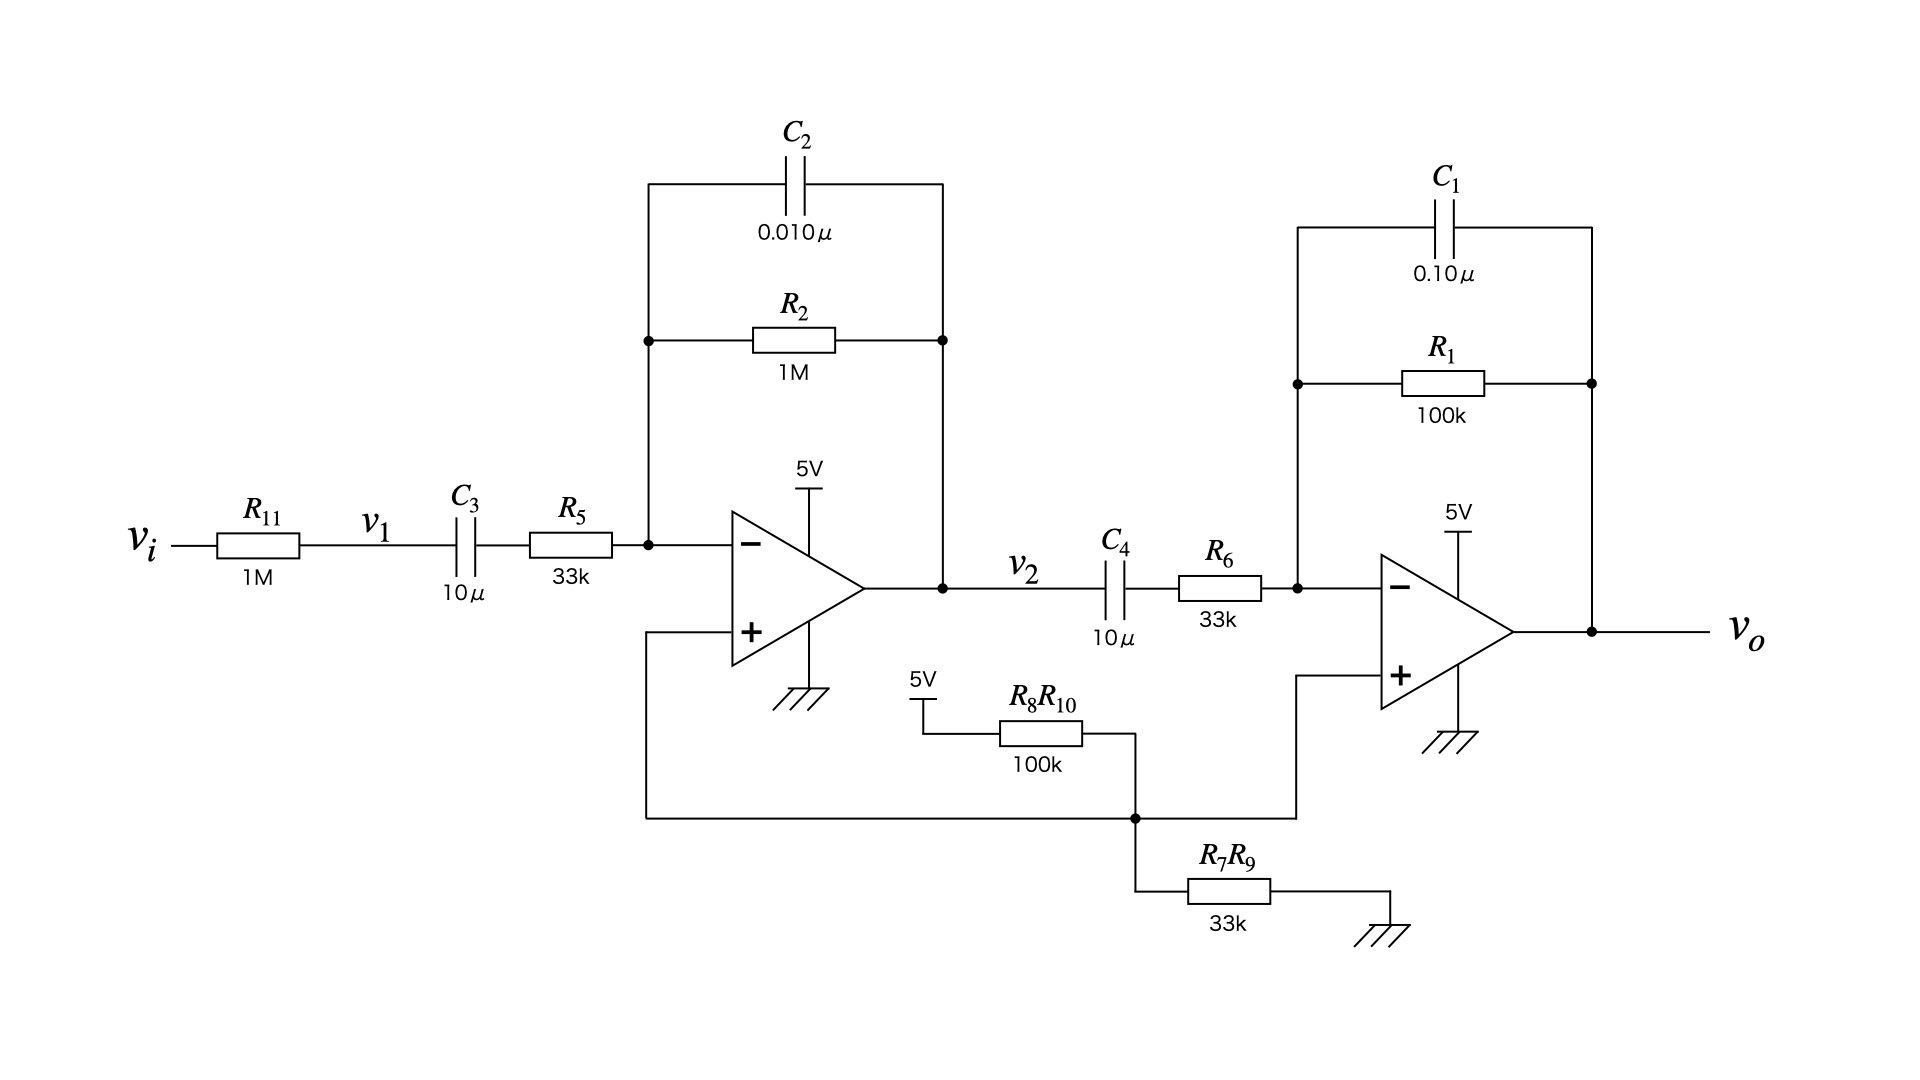
\includegraphics[width=1\linewidth]{fig_work_A/1_fig.jpg}
  \caption{ワークA-1 回路図}
  \label{fig:1_fig}
\end{figure}
\begin{figure}[H]
  \centering
  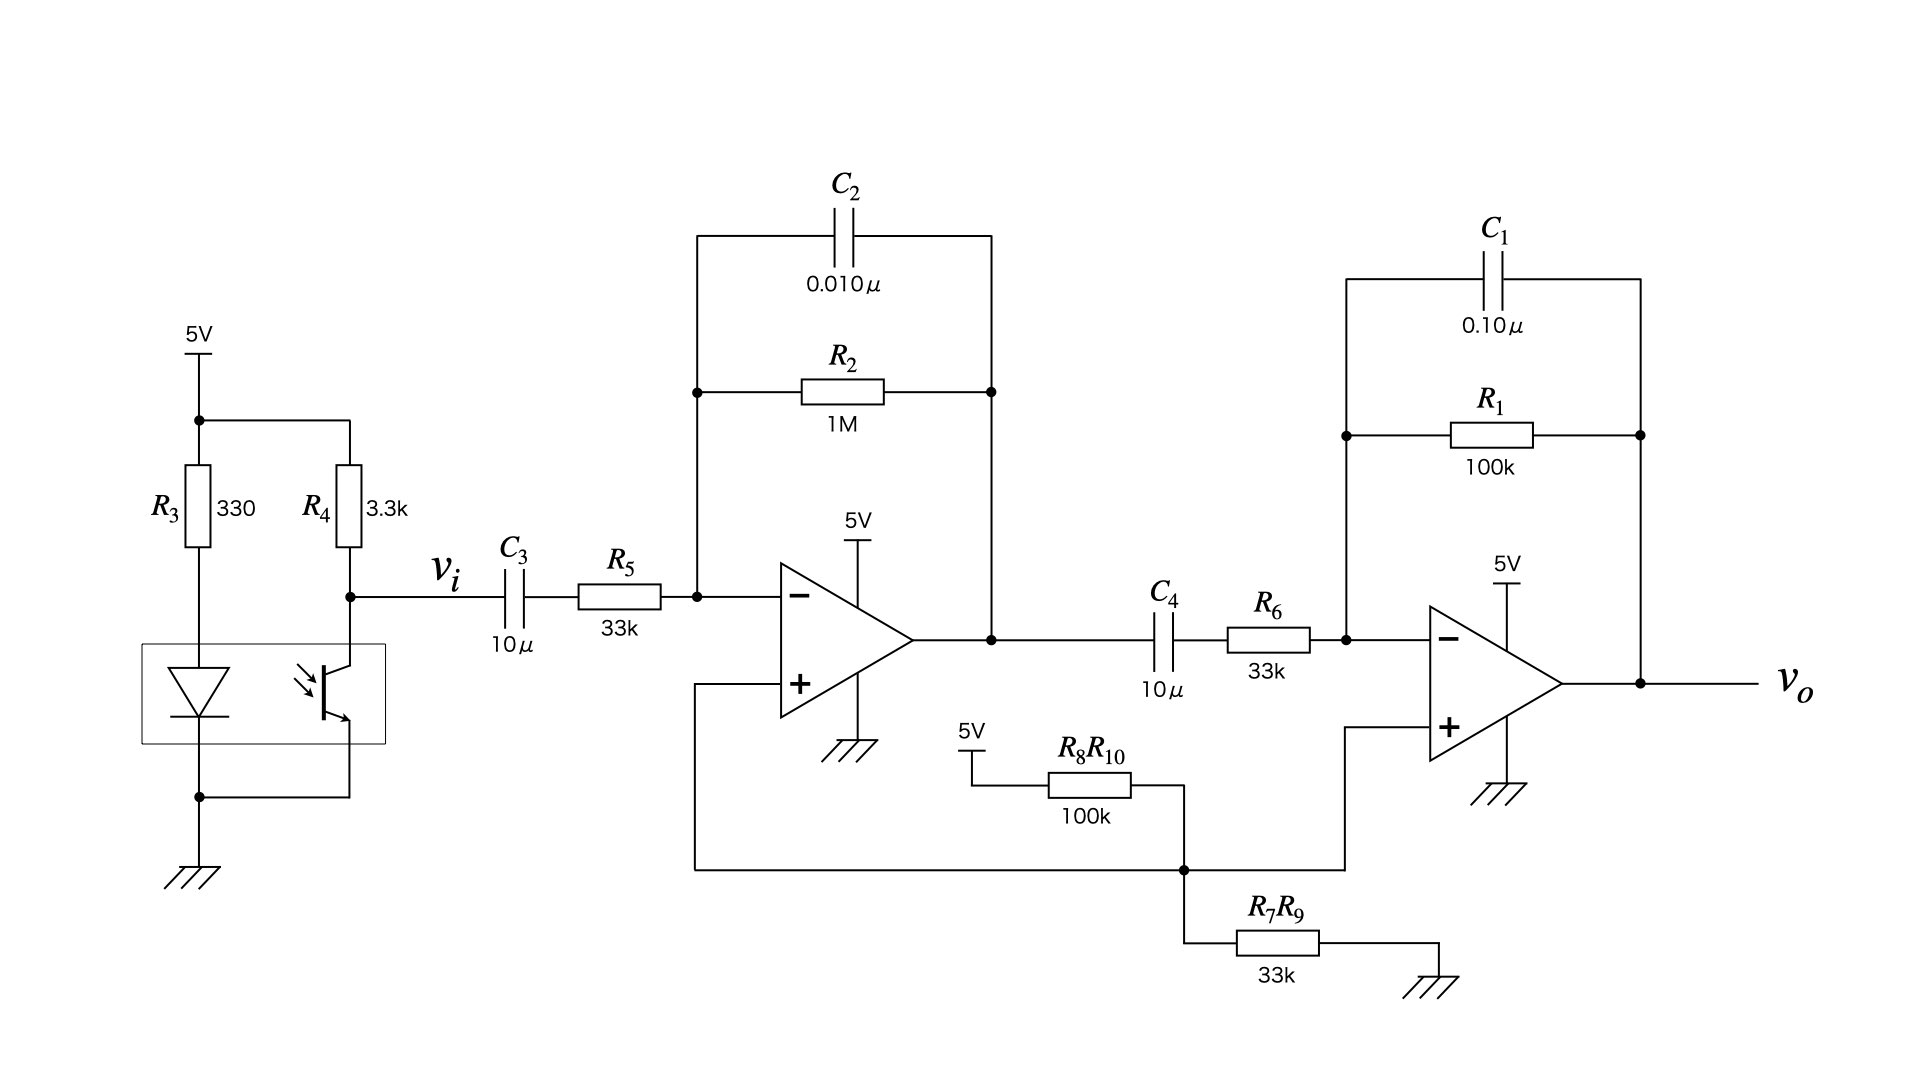
\includegraphics[width=1\linewidth]{fig_work_A/2_fig.jpg}
  \caption{ワークA-2 回路図}
  \label{fig:2_fig}
\end{figure}

\subsection{ワークA-1: センサ後段回路}
設計した増幅・フィルタ回路の特性を評価するため，図\ref{fig:1_fig}に示す回路を図\ref{fig:1_pic}のように実装した．
入力端子には，波形出力デバイス(ATOM Lite)を1M$\Omega$の抵抗($R_{11}$)を介して接続した．
\begin{figure}[H]
  \centering
  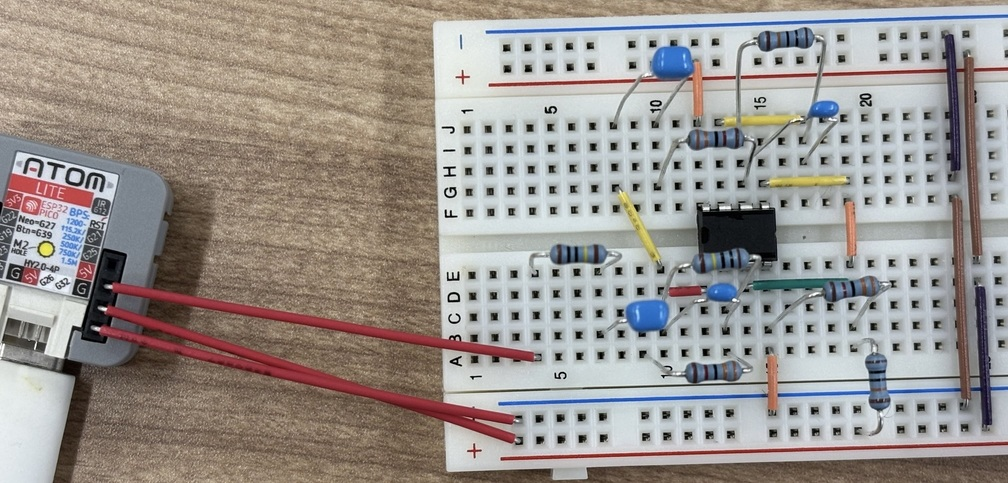
\includegraphics[width=0.9\linewidth]{fig_work_A/1_pic.jpg}
  \caption{ワークA-1 実装回路}
  \label{fig:1_pic}
\end{figure}

まず，回路の各増幅段が設計通りに動作することを確認するため，1Hzの正弦波を入力し，以下の3点についてオシロスコープで観測を行う．
\begin{enumerate}
  \item 一段目(-30.3倍)の動作確認: 回路の入力($v_1$)と一段目の出力($v_2$)を観測し，増幅率と位相の反転を確認する．
  \item 二段目(-3.03倍)の動作確認: 一段目の出力($v_2$)と回路全体の出力($v_o$)を観測し，増幅率と位相の反転を確認する．
  \item 増幅回路全体(91.8倍)の動作確認: 回路の入力($v_1$)と出力($v_o$)を観測し，全体の増幅率を確認する．
\end{enumerate}

次に，4種類の波形(1Hz正弦波，1Hzと100Hzの合成波，1Hzと7Hzの合成波，脈波)をそれぞれ入力し，入力($v_1$)と出力($v_o$)をオシロスコープで観測する．
観測では，各波形の周期，振幅，および入出力間の時間差を測定する．

\newpage

\subsection{ワークA-2: 脈拍検出回路}
ワークA-1の回路の入力部を，設計した脈拍検出回路に置き換え，図\ref{fig:2_fig}に示す回路を図\ref{fig:2_pic}のように実装した．
\begin{figure}[H]
  \centering
  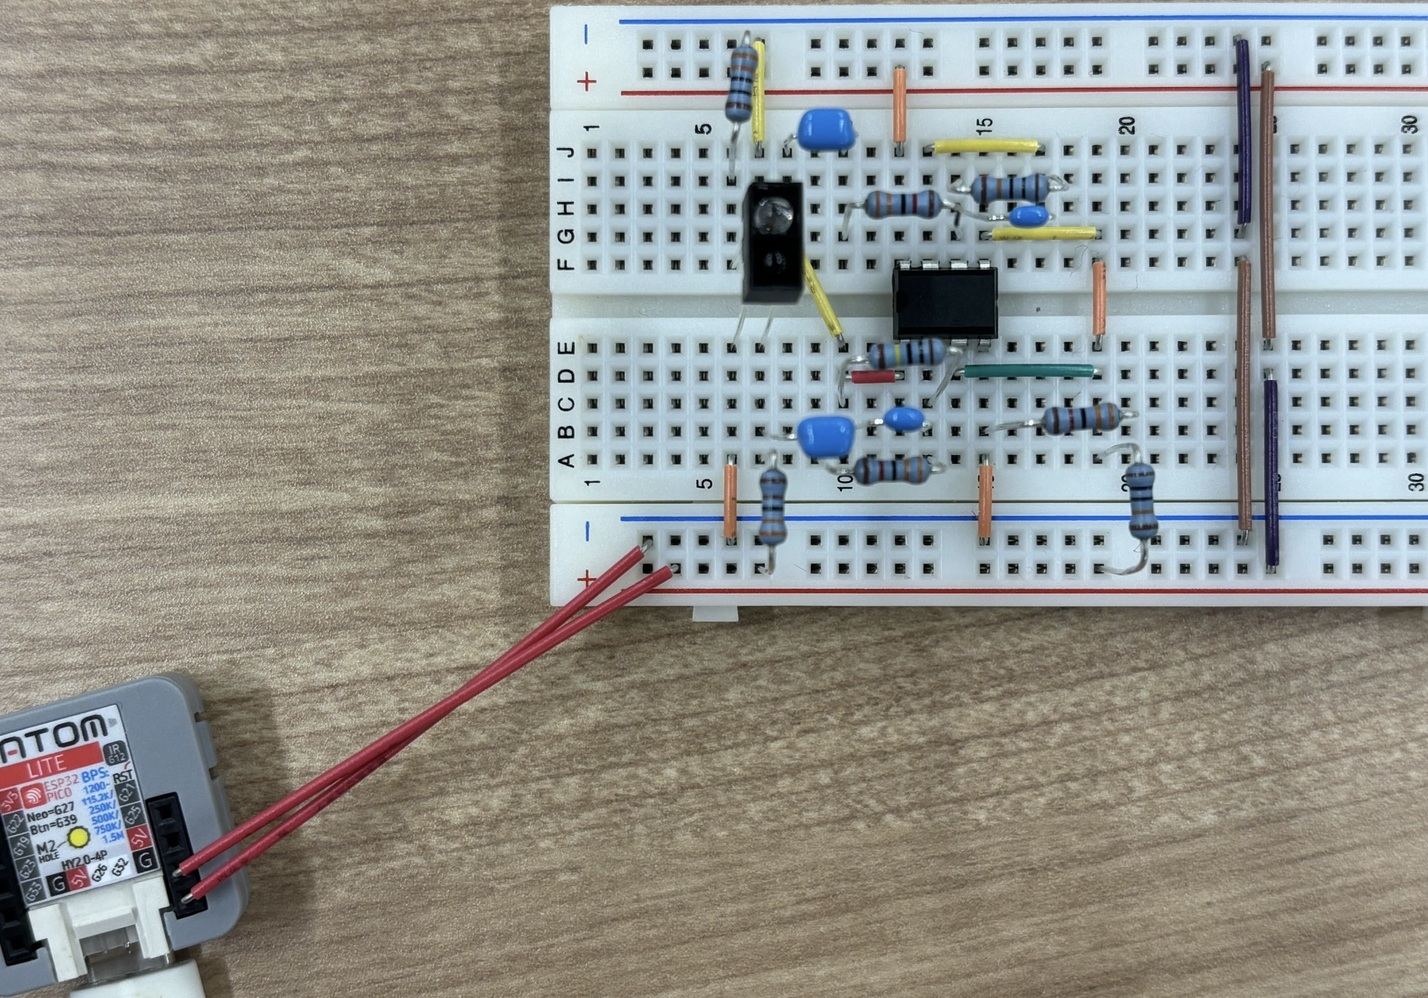
\includegraphics[width=0.9\linewidth]{fig_work_A/2_pic.jpg}
  \caption{ワークA-2 実装回路}
  \label{fig:2_pic}
\end{figure}
フォトリフレクタに指を置き，オシロスコープで脈波検出回路から出力された脈波($v_i$)と最終的な脈波($v_o$)を観測する．
この際，出力電圧の振幅が仕様(1V以上，4V未満)を満たすことを確認する．


\newpage

\section{結果} 
%% 実験から得られた結果を，目的や方法を理解した上で，重要データを外す
%% ことなく，要領よくまとめてください．
%% 
%% 結果（数値）は，（自分はポイントを理解しているということをアピール
%% しながら）視認性（一覧性）を高めて報告することが求められる．この意
%% 味で，要領よくまとめられた表が望ましい．決して，文章の中にバラバラ
%% に埋没させて，読み手がどこに書いているか分かりにくい（書き手にとっ
%% ては都合のよい）記載するものではない点に注意する．
%% 
%% 
%% 結果をまとめた表の例
%% ただし，ワーク前の説明で話した通り，
%%   - 一次データ（生データ）
%%   - 計器パラメータ（レンジなど）
%%   - 中間算出値（二次以上の高次データ）
%%   - 周期，時間差，入力電位，出力電位（必須データ）
%%   - 手順書の課題4.で求められるデータ（必須データ）
%% を記録した表に書き換えて，結果報告してください．

\subsection{ワークA-1: センサ後段回路}
\subsubsection{各増幅段の動作確認}
回路の各増幅段が設計通りに動作することを確認するため，1Hzの正弦波を入力し，各段の入出力波形を観測した．
一段目(-30.3倍)および二段目(-3.03倍)，並びに一段目と二段目を合わせた回路全体のオシロスコープ画面を，
それぞれ図\ref{fig:1_green_v1v2}，図\ref{fig:1_green_v2vo}，図\ref{fig:1_green_v1vo}に示す．
\begin{figure}[H]
  \centering
  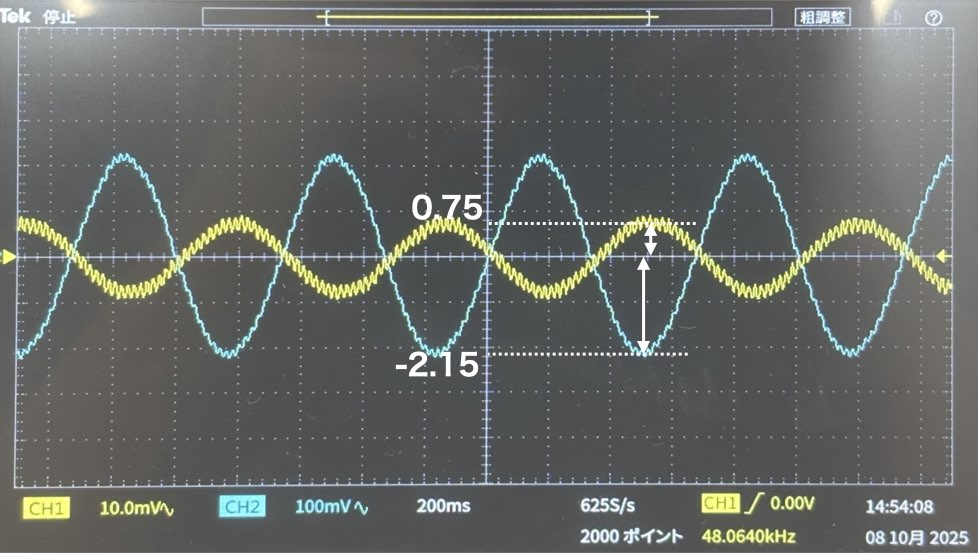
\includegraphics[width=0.8\linewidth]{fig_work_A/1_green_v1v2.jpg}
  \caption{一段目増幅回路の入出力波形(黄:$v_1$，青:$v_2$)．図中の書き込みは，表\ref{tab:result1-1}の一段目の目盛り読み取り値を示す．}
  \label{fig:1_green_v1v2}
\end{figure}
\begin{figure}[H]
  \centering
  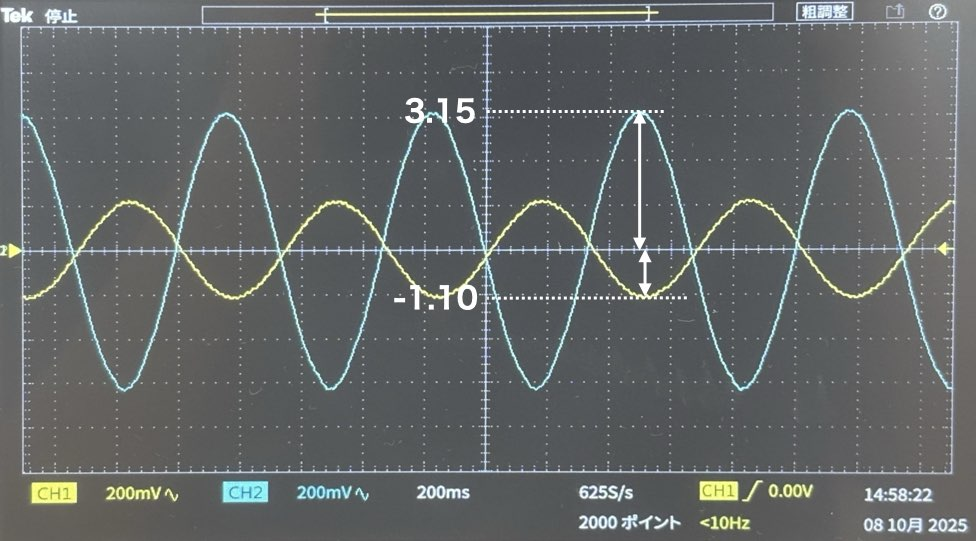
\includegraphics[width=0.8\linewidth]{fig_work_A/1_green_v2vo.jpg}
  \caption{二段目増幅回路の入出力波形(黄:$v_2$，青:$v_o$)．図中の書き込みは，表\ref{tab:result1-1}の二段目の目盛り読み取り値を示す．}
  \label{fig:1_green_v2vo}
\end{figure}
\begin{figure}[H]
  \centering
  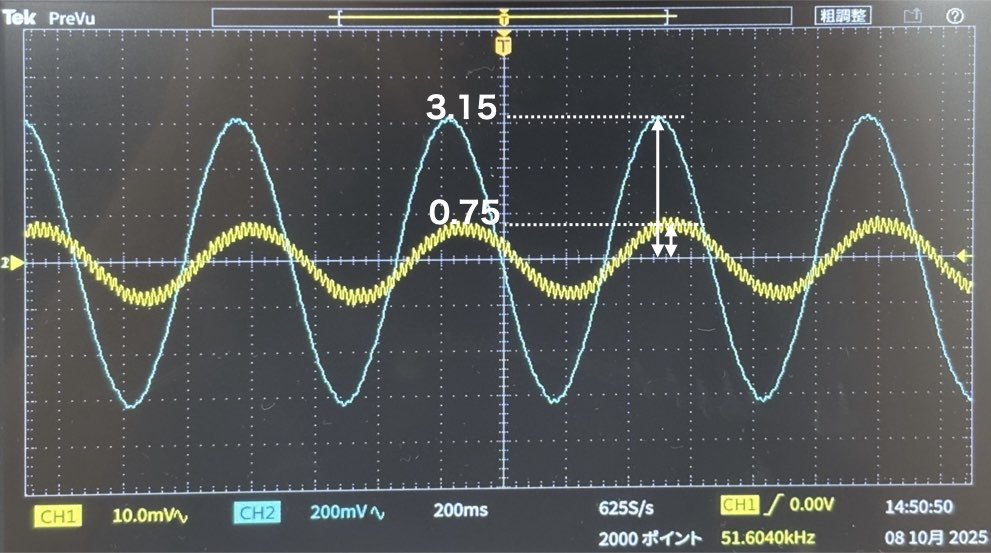
\includegraphics[width=0.8\linewidth]{fig_work_A/1_green_v1vo.jpg}
  \caption{二段反転増幅回路の入出力波形(黄:$v_1$，青:$v_o$)．図中の書き込みは，表\ref{tab:result1-1}の回路全体の目盛り読み取り値を示す．}
  \label{fig:1_green_v1vo}
\end{figure}
測定値から算出した各段の増幅率を表\ref{tab:result1-1}にまとめる．
\begin{table}[H]
  \caption{各増幅段の増幅率}
  \centering
  \begin{tabular}{|c|c|c|c|c|c|c|}
    \hline
    \multirow{2}{*}{増幅段} & \multirow{2}{*}{信号} & スケール & 読み取り値 & 測定電圧 & 測定増幅率 & 設計増幅率 \\
     & & [V/div] & [div] & [mV] & [倍] & [倍] \\
    \hline \hline
    \multirow{2}{*}{一段目} & 入力($v_1$) & 10.0m & 0.75 & 7.50 & \multirow{2}{*}{-28.6} & \multirow{2}{*}{-30.3} \\
    \cline{2-5}
     & 出力($v_2$) & 100m & -2.15 & -215 & & \\
    \hline
    \multirow{2}{*}{二段目} & 入力($v_2$) & 200m & -1.10 & -220 & \multirow{2}{*}{-2.86} & \multirow{2}{*}{-3.03} \\
    \cline{2-5}
     & 出力($v_o$) & 200m & 3.15 & 630 & & \\
    \hline
    \multirow{2}{*}{回路全体} & 入力($v_1$) & 10.0m & 0.75 & 7.50 & \multirow{2}{*}{84.0} & \multirow{2}{*}{91.8} \\
    \cline{2-5}
     & 出力($v_o$) & 200m & 3.15 & 630 & & \\
    \hline
  \end{tabular}
  \label{tab:result1-1}
\end{table}

\newpage


\subsubsection{回路全体の周波数特性評価}
回路全体の特性を評価するため，4種類の波形を入力した際のオシロスコープ画面を図\ref{fig:1_green}，図\ref{fig:1_red}，図\ref{fig:1_red2}，
図\ref{fig:1_blue}，図\ref{fig:1_blue2}，図\ref{fig:1_purple}，図\ref{fig:1_purple2}に示す．
\begin{figure}[H]
  \centering
  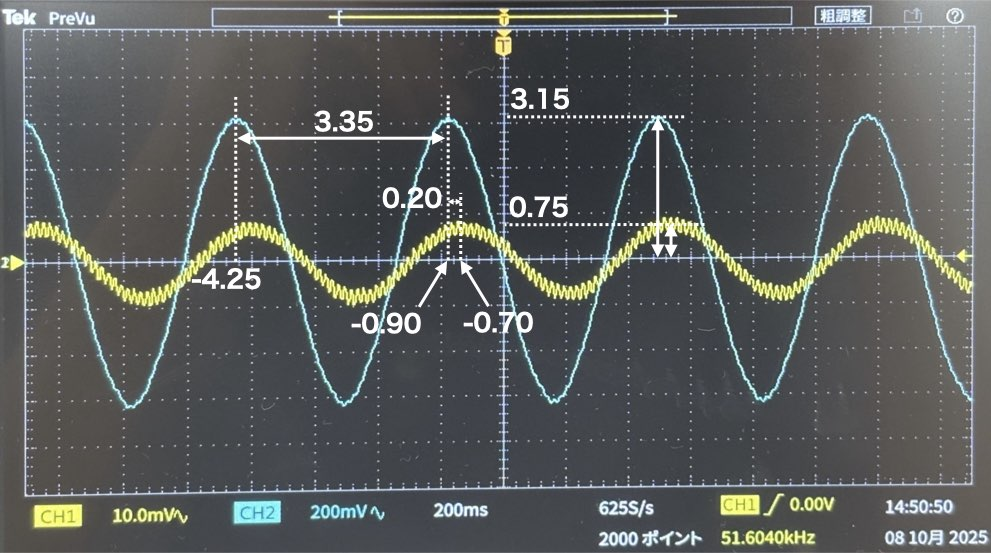
\includegraphics[width=0.9\linewidth]{fig_work_A/1_green.jpg}
  \caption{1Hz正弦波(黄:$v_1$，青:$v_o$)．図中の書き込みは，表\ref{tab:result1-2}の波形1の目盛り読み取り値を示す．}
  \label{fig:1_green}
\end{figure}
\begin{figure}[H]
  \centering
  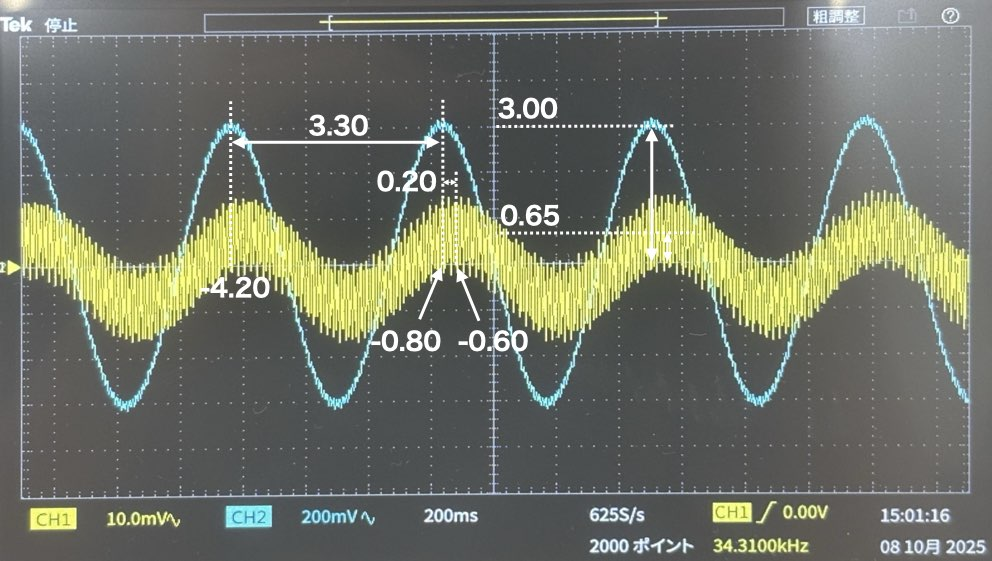
\includegraphics[width=0.9\linewidth]{fig_work_A/1_red.jpg}
  \caption{1Hzと100Hzの合成波(黄:$v_1$，青:$v_o$)．図中の書き込みは，表\ref{tab:result1-2}の波形2，低周波成分の目盛り読み取り値を示す．}
  \label{fig:1_red}
\end{figure}
\begin{figure}[H]
  \centering
  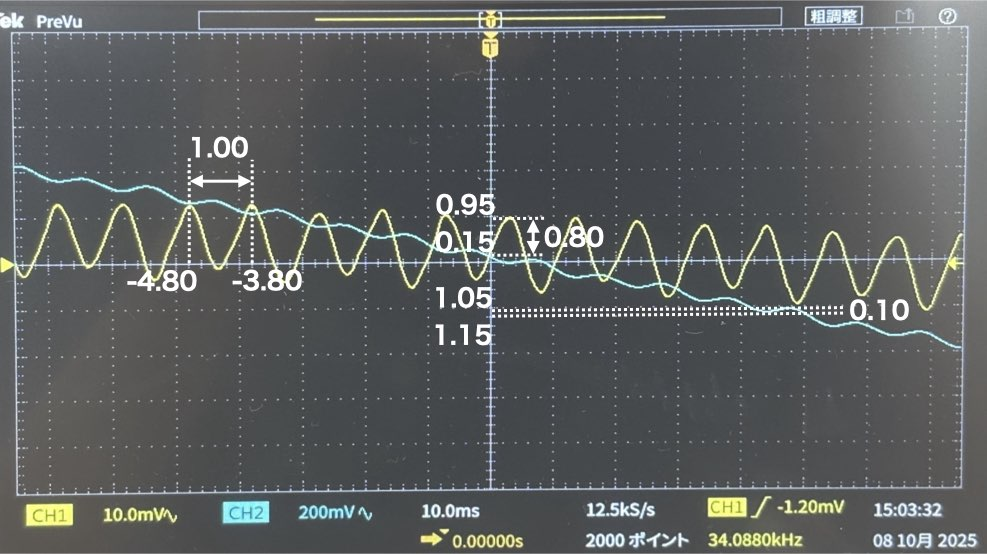
\includegraphics[width=0.9\linewidth]{fig_work_A/1_red2.jpg}
  \caption{時間軸を拡大した1Hzと100Hzの合成波(黄:$v_1$，青:$v_o$)．図中の書き込みは，表\ref{tab:result1-2}の波形2，高周波成分の目盛り読み取り値を示す．}
  \label{fig:1_red2}
\end{figure}
\begin{figure}[H]
  \centering
  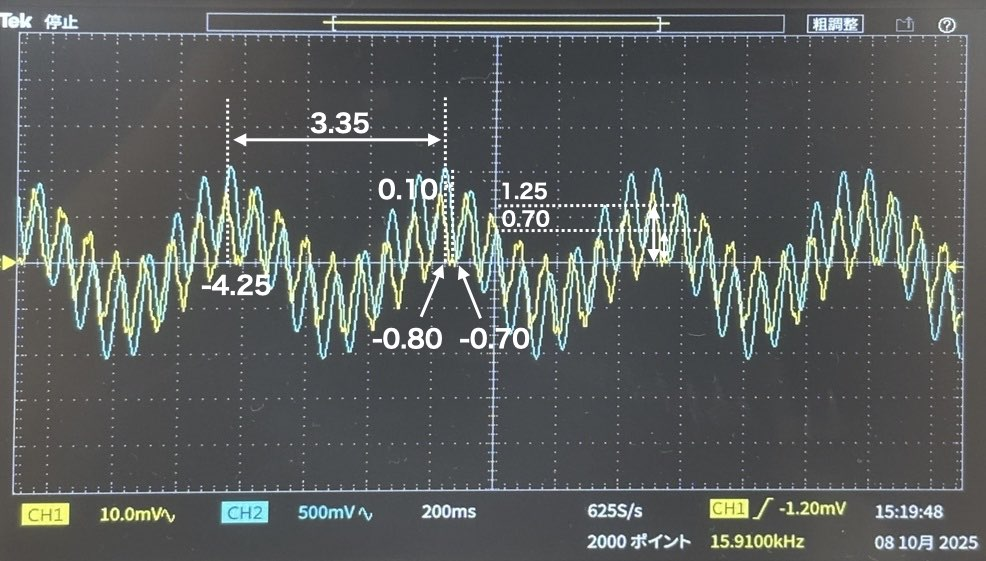
\includegraphics[width=0.9\linewidth]{fig_work_A/1_blue.jpg}
  \caption{1Hzと7Hzの合成波(黄:$v_1$，青:$v_o$)．図中の書き込みは，表\ref{tab:result1-2}の波形3，低周波成分の目盛り読み取り値を示す．}
  \label{fig:1_blue}
\end{figure}
\begin{figure}[H]
  \centering
  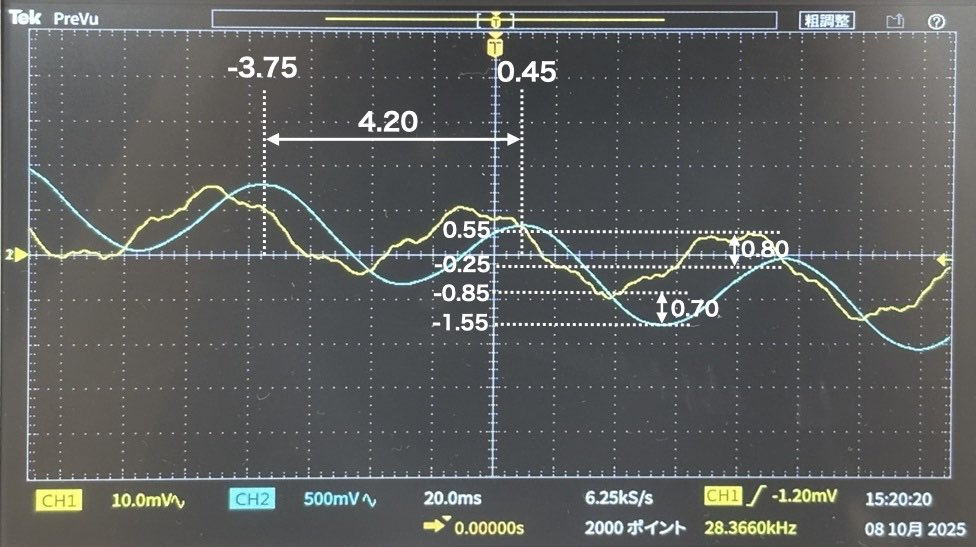
\includegraphics[width=0.9\linewidth]{fig_work_A/1_blue2.jpg}
  \caption{時間軸を拡大した1Hzと7Hzの合成波(黄:$v_1$，青:$v_o$)．図中の書き込みは，表\ref{tab:result1-2}の波形3，高周波成分の目盛り読み取り値を示す．}
  \label{fig:1_blue2}
\end{figure}
\begin{figure}[H]
  \centering
  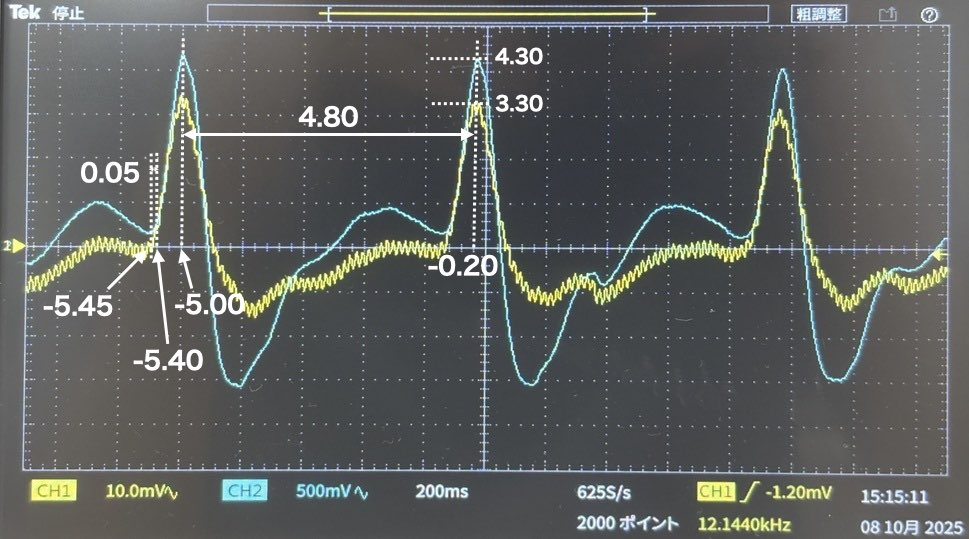
\includegraphics[width=0.9\linewidth]{fig_work_A/1_purple.jpg}
  \caption{脈波(黄:$v_1$，青:$v_o$)．図中の書き込みは，表\ref{tab:result1-2}の波形4，低周波成分の目盛り読み取り値を示す．}
  \label{fig:1_purple}
\end{figure}
\begin{figure}[H]
  \centering
  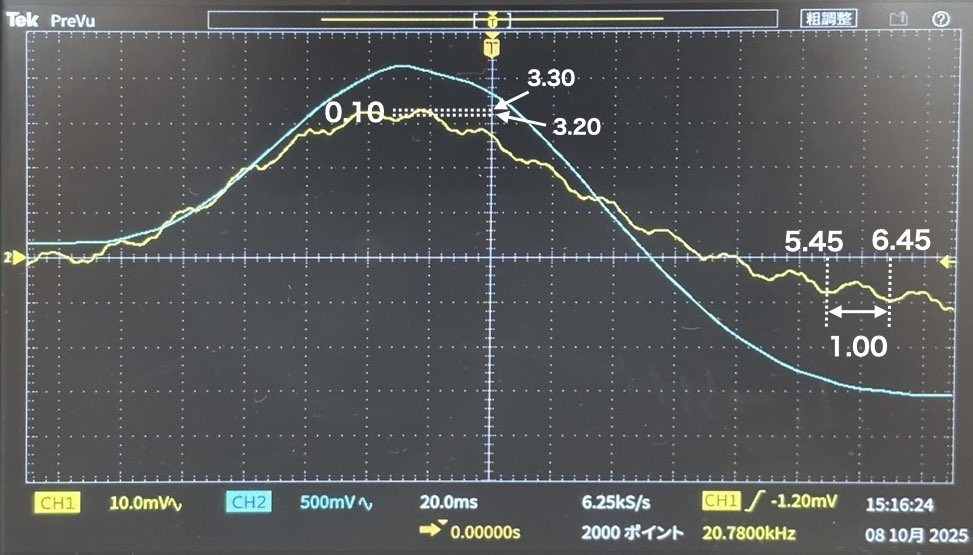
\includegraphics[width=0.9\linewidth]{fig_work_A/1_purple2.jpg}
  \caption{時間軸を拡大した脈波(黄:$v_1$，青:$v_o$)．図中の書き込みは，表\ref{tab:result1-2}の波形4，高周波成分の目盛り読み取り値を示す．}
  \label{fig:1_purple2}
\end{figure}
各波形を観測した際の計測結果を表\ref{tab:result1-2}にまとめ，
表\ref{tab:result1-2}の計測結果から算出した数値を表\ref{tab:result1-3}にまとめる．
\begin{table}[H]
  \caption{波形出力デバイスの計測における読み取り値(一次データ)}
  \centering
  \begin{tabular}{|c|c|c|c|c|c|c|c|}
    \hline
    \multirow{2}{*}{波形} & \multirow{2}{*}{成分} & \multirow{2}{*}{信号} & スケール & 読み取り値 & \multirow{2}{*}{項目} & スケール & 読み取り値 \\[-4pt]
    & & & [mV/div] & [div] & & [ms/div] & [div] \\
    \hline \hline
    \multirow{2}{*}{1} & \multirow{2}{*}{低周波} & 入力 ($v_1$) & 10.0 & 0.75 & 周期 & 200 & 3.35 \\
    \cline{3-8}
    & & 出力 ($v_o$) & 200 & 3.15 & 時間差 & 200 & 0.20 \\
    \hline
    \multirow{4}{*}{2} & \multirow{2}{*}{低周波} & 入力 ($v_1$) & 10.0 & 0.65 & 周期 & 200 & 3.30 \\
    \cline{3-8}
    & & 出力 ($v_o$) & 200 & 3.00 & 時間差 & 200 & 0.20 \\
    \cline{2-8}
    & \multirow{2}{*}{高周波} & 入力 ($v_1$) & 10.0 & 0.80 & \multirow{2}{*}{周期} & \multirow{2}{*}{10.0} & \multirow{2}{*}{1.00} \\
    \cline{3-5}
    & & 出力 ($v_o$) & 200 & 0.10 & & & \\
    \hline
    \multirow{4}{*}{3} & \multirow{2}{*}{低周波} & 入力 ($v_1$) & 10.0 & 0.70 & 周期 & 200 & 3.35 \\
    \cline{3-8}
    & & 出力 ($v_o$) & 500 & 1.25 & 時間差 & 200 & 0.10 \\
    \cline{2-8}
    & \multirow{2}{*}{高周波} & 入力 ($v_1$) & 10.0 & 0.80 & \multirow{2}{*}{周期} & \multirow{2}{*}{20.0} & \multirow{2}{*}{4.20} \\
    \cline{3-5}
    & & 出力 ($v_o$) & 500 & 0.70 & & & \\
    \hline
    \multirow{4}{*}{4} & \multirow{2}{*}{低周波} & 入力 ($v_1$) & 10.0 & 3.30 & 周期 & 200 & 4.80 \\
    \cline{3-8}
    & & 出力 ($v_o$) & 500 & 4.30 & 時間差 & 200 & 0.05 \\
    \cline{2-8}
    & \multirow{2}{*}{高周波} & 入力 ($v_1$) & 10.0 & 0.10 & \multirow{2}{*}{周期} & \multirow{2}{*}{20.0} & \multirow{2}{*}{1.00} \\
    \cline{3-5}
    & & 出力 ($v_o$) & 500 & (測定不能) & & & \\
    \hline
  \end{tabular}
  \label{tab:result1-2}
\end{table}
\begin{table}[H]
  \caption{一次データに基づく算出結果(高次データ)}
  \centering
  \small
  \begin{tabular}{|c|c|c|c|c|c|c|c|c|c|}
    \hline
    \multirow{2}{*}{波形} & \multirow{2}{*}{成分} & 時間差 & ~周期~ & 測定周波数 & 設計周波数 & $v_1$振幅 & $v_o$振幅 & 増幅率 & 脈拍数 \\[-4pt]
    & & [ms] & [ms] & [Hz] & [Hz] & [mV] & [mV] & [倍] & [bpm] \\
    \hline \hline
    1 & 低周波 & 40.0 & 670 & 1.49 & 1 & 7.50 & 630 & 84.0 & - \\
    \hline
    \multirow{2}{*}{2} & 低周波 & 40.0 & 660 & 1.51 & 1 & 6.50 & 600 & 92.3 & - \\
    \cline{2-10}
    & 高周波 & - & 10.0 & 100 & 100 & 8.00 & 20.0 & 2.50 & - \\
    \hline
    \multirow{2}{*}{3} & 低周波 & 20.0 & 670 & 1.49 & 1 & 7.00 & 625 & 89.3 & - \\
    \cline{2-10}
    & 高周波 & - & 84.0 & 11.9 & 7 & 8.00 & 350 & 43.8 & - \\
    \hline
    \multirow{2}{*}{4} & 低周波 & 10.0 & 960 & 1.04 & - & 33.0 & $2.15 \times 10^3$ & 65.2 & 62.5 \\
    \cline{2-10}
    & 高周波 & - & 20.0 & 50.0 & - & 1.00 & (測定不能) & (測定不能) & - \\
    \hline
  \end{tabular}
  \label{tab:result1-3}
\end{table}


\subsection{ワークA-2: 脈拍検出回路の評価}
最終的に，フォトリフレクタに指を置き，脈拍を測定した．
オシロスコープで観測した脈波の波形を図\ref{fig:2_result}に示す．
\begin{figure}[H]
  \centering
  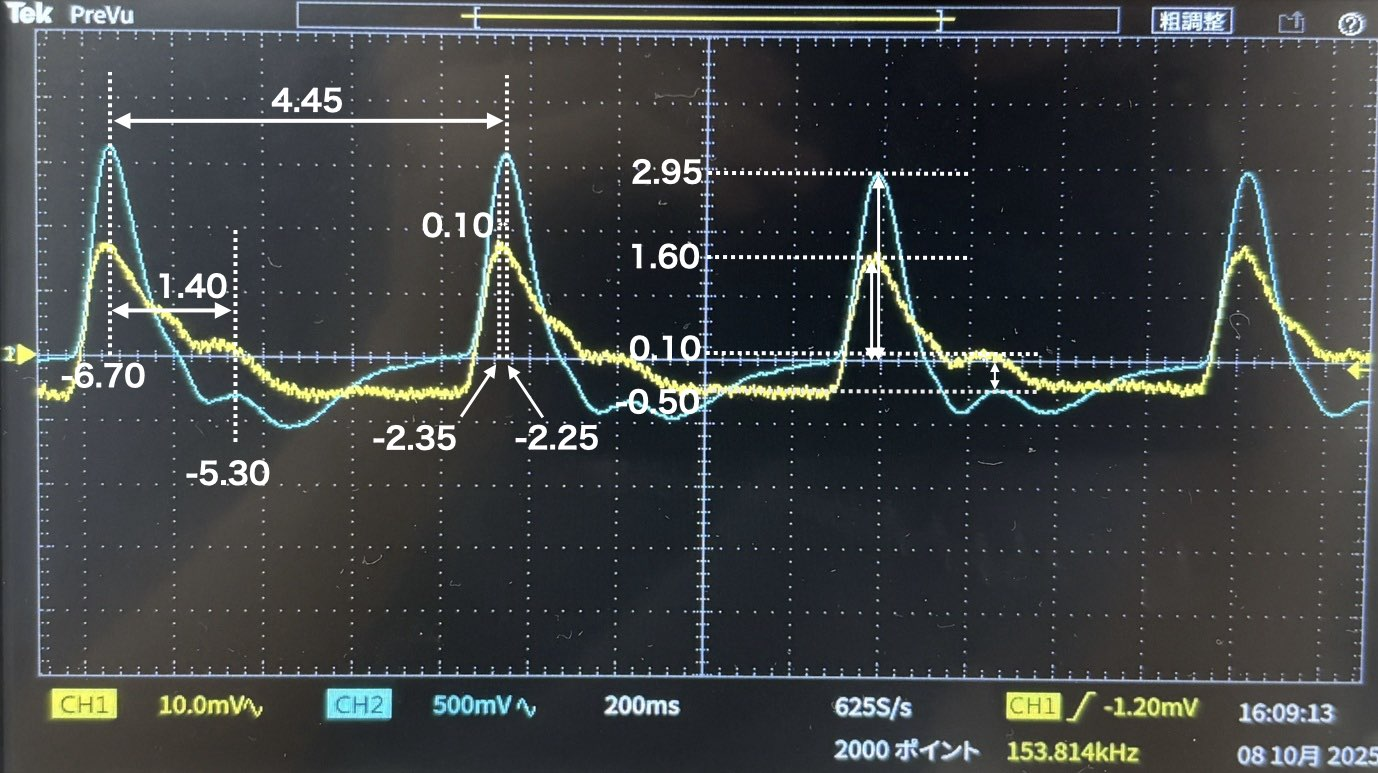
\includegraphics[width=0.9\linewidth]{fig_work_A/2_result.jpg}
  \caption{測定した自身の脈波(黄:$v_i$，青:$v_o$)．図中の書き込みは，表\ref{tab:result2-1}の主脈波および副脈波の目盛り読み取り値を示す．}
  \label{fig:2_result}
\end{figure}
\newpage
また，観測された波形の計測結果を表\ref{tab:result2-1}にまとめ，
表\ref{tab:result2-1}の計測結果から算出した数値を表\ref{tab:result2-2}にまとめる．
\begin{table}[H]
  \caption{脈拍測定における読み取り値(一次データ)}
  \centering
  \begin{tabular}{|c|c|c|c|}
    \hline
    \multirow{2}{*}{測定項目} & \multirow{2}{*}{信号} & \multicolumn{2}{c|}{電圧測定} \\
    \cline{3-4}
    & & スケール [mV/div] & 読み取り値 [div] \\
    \hline
    \multirow{2}{*}{主脈波} & 入力($v_i$) & 10.0 & 1.60 \\
    \cline{2-4}
     & 出力($v_o$) & 500 & 2.95 \\
    \hline
    \multirow{2}{*}{副脈波} & 入力($v_i$) & 10.0 & 0.10 \\
    \cline{2-4}
     & 出力($v_o$) & 500 & -0.50 \\
    \hline \hline
    \multirow{2}{*}{測定項目} & \multirow{2}{*}{項目} & \multicolumn{2}{c|}{時間測定} \\
    \cline{3-4}
     & & スケール [ms/div] & 読み取り値 [div] \\
    \hline
    主脈波 & 周期 & 200 & 4.45 \\
    \cline{2-4}
    と & 時間差 & 200 & 0.10 \\
    \cline{2-4}
    副脈波 & 間隔 & 200 & 1.40 \\
    \hline
  \end{tabular}
  \label{tab:result2-1}
\end{table}
\begin{table}[H]
  \caption{一次データに基づく算出結果(高次データ)}
  \centering
  \begin{tabular}{|c|c|c|c|c|c|c|c|c|}
    \hline
    \multirow{2}{*}{信号} & $v_i$振幅 & $v_o$振幅 & 増幅率 & 時間差 & 周期 & 周波数 & 脈拍数 & ~間隔~ \\[-4pt]
     & {[mV]} & {[mV]} & {[倍]} & {[ms]} & {[ms]} & {[Hz]} & {[bpm]} & {[ms]} \\
    \hline \hline
    主脈波 & 16.0 & 1475 & 92.2 & \multirow{2}{*}{20.0} & \multirow{2}{*}{890} & \multirow{2}{*}{1.12} & \multirow{2}{*}{67.4} & \multirow{2}{*}{280} \\
    \cline{1-4}
    副脈波 & 1.00 & -250 & -250 & & & & & \\
    \hline
  \end{tabular}
  \label{tab:result2-2}
\end{table}
\newpage
さらに，フォトリフレクタに指を置いた直後の波形を図\ref{fig:2_result2}に示し，図\ref{fig:2_result2}で観測された出力($v_o$)の遅延時間を表\ref{tab:result2-3}にまとめる．
\begin{figure}[H]
  \centering
  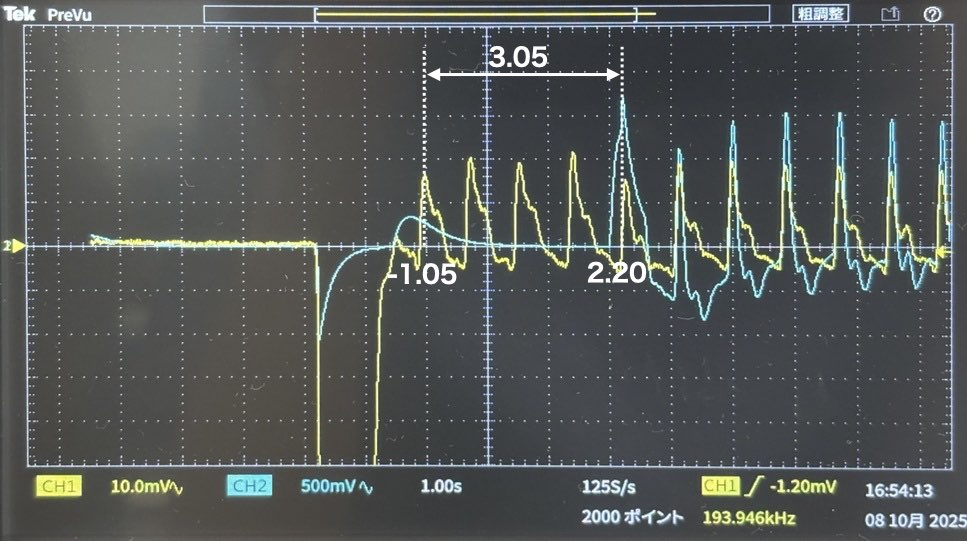
\includegraphics[width=0.9\linewidth]{fig_work_A/2_result2.jpg}
  \caption{フォトリフレクタに指を置いた直後の波形(黄:$v_i$，青:$v_o$)．図中の書き込みは，表\ref{tab:result2-3}の入力($v_i$)で波形が現れてから出力($v_o$)で波形が現れるまでの遅延時間の目盛り読み取り値を示す．}
  \label{fig:2_result2}
\end{figure}
\begin{table}[H]
  \caption{入力($v_i$)で波形が現れてから出力($v_o$)で波形が現れるまでの遅延時間}
  \centering
  \begin{tabular}{|c|c|c|}
    \hline
    スケール [s/div] & 読み取り値 [div] & 遅延時間[s] \\
    \hline \hline
    1.00 & 3.05 & 3.05 \\
    \hline
  \end{tabular}
  \label{tab:result2-3}
\end{table}


%% 必ず下記のものは写真を撮るなどして図として報告書に記載してください．
%% 実装した回路
%% オシロスコープに表示された自分の脈波

%\begin{figure}[ht]
%\begin{center}
%\includegraphics[width=0.95\textwidth,clip]{fig_work_A/}
%\end{center}
%\caption{\textgt{
%    図の内容を表す適切なキャプションをつける
%}}
%\label{sample}
%\end{figure}



\section{考察}
%% 手順書の「４ 考察」であげた３項目を含み，結果（数値）に対する自分の
%% 考えを述べよ．
%% 感想とならないよう，数値に基づいた定量的な考察となるように注意する．


\subsection{増幅率と周波数特性}
設計した回路の増幅およびフィルタ性能について，測定結果から考察する．
まず，誤差の主な原因として，使用した抵抗器(許容差±5\%)およびコンデンサ(許容差±10\%)の部品個体差が複合的に作用したことが考えられる．

次に，回路の各増幅段の動作を確認した．
表\ref{tab:result1-1}より，一段目の測定増幅率は-28.6倍(設計値-30.3倍)，二段目は-2.86倍(設計値-3.03倍)となり，
各段において設計値に非常に近い増幅率が得られた．これは，各増幅段が個別にほぼ設計通りに動作していることを示している．
また，増幅回路全体の測定増幅率は84.0倍(設計値91.8倍)となり，設計値より約-8.5\%の誤差が生じたものの，
部品の個体差を考慮すれば，回路全体としてもほぼ設計通りに機能していることを示している．

続いて，回路全体の周波数特性を，各周波数における増幅率から評価する．
表\ref{tab:result1-3}より，通過可能な周波数の範囲内にある1.49Hzや1.51Hzの信号に対する増幅率は，波形1で84.0倍，波形2で92.3倍，波形3で89.3倍であり，設計増幅率91.8倍に近い値を示した．
したがって，回路が通過帯域内の信号を意図通りに増幅していることが確認できた．

さらに，高周波数成分に対する増幅率を評価する．
表\ref{tab:result1-3}より，上限周波数16Hzに近い11.9Hz成分(波形3)では，増幅率が43.8倍に低下していた．
この結果は偶然誤差の影響も考えられるが，フィルタの減衰効果が上限周波数で急に始まるのではなく，
通過可能な周波数の範囲内であっても，上限周波数に近づくにつれて増幅率が低下し始めることも考えられる．
また，上限周波数を大幅に超える100Hz成分(波形2)では，増幅率がわずか2.50倍にまで低下し，50.0Hz(波形4)に至っては，出力側($v_o$)で観測が不可能なレベルになっていた．
この結果は，設計した回路が高周波ノイズを効果的に減衰させる能力を持つことを示している．

以上の結果から，測定された増幅率は周波数によって変動するものの，それは設計したバンドパスフィルタの特性を反映したものであり，
部品の許容差を考慮すれば，本回路はほぼ設計通りの増幅およびフィルタ性能を持つと結論付けられる．



\subsection{脈拍検出回路}
まず，表\ref{tab:result2-2}より，測定した脈拍数は67.4bpmであり，一般的な安静時の脈拍数として妥当な値である\cite{workA_脈拍数}．
このとき，回路全体の増幅率は92.2倍となり，設計値91.8倍とほぼ一致した．
したがって，ワークA-1で性能を評価した回路が，実際の微弱な生体信号(脈波)に対しても有効に機能し，
観測に適したレベルまで増幅できることが実証された．

次に，観測された図\ref{fig:2_result}の脈波の波形には，最も振幅の大きな主脈波の280ms後に，振幅の小さな副脈波が確認できる．
表\ref{tab:result2-2}からも，これは単なるノイズとは異なる周期的な特徴であることがわかる．
本回路が，主となる脈の周期成分だけでなく，それに重複したこのような微細な電圧変動までも増幅できていることは，
設計したフィルタ増幅回路が十分な感度と性能を有していることを示している．

一方で，表\ref{tab:result2-2}において，副脈波の増幅率は-250倍となった．
回路の設計増幅率は正の値(+91.8倍)であり，主脈派はそれに沿った正常な増幅率(+92.2倍)であることから，この測定結果は矛盾している．
この原因として，測定時の基準電圧の設定に問題があった可能性が考えられる．
オシロスコープの時間軸（中央線）を0V基準として読み取りを行ったが，実際の信号のグラウンドがこの基準線と正確に一致していなかった可能性がある．
そのため，本来は$v_o$と同様に基準線より下に振れていたはずの$v_i$の副脈波が，基準レベルのずれにより，見かけ上プラスの値として読み取られてしまい，
回路の増幅特性とは矛盾した測定結果になったと考察される．

\newpage

さらに，図\ref{fig:2_result2}では，フォトリフレクタに指を置いた直後の応答が観測されている．
入力側($v_i$)では脈波がすぐに検出されているにもかかわらず，出力側($v_o$)で初めて検出されたのは，表\ref{tab:result2-3}より，入力側($v_i$)で検出された3.05秒後であった．
これには，コンデンサが関係していると考えられる．
指を置いた瞬間にセンサの電圧レベルが大きく変化するため，コンデンサが変化後の電圧に合わせて充電されるまでに一定の時間が必要となる．
これが完了するまでの間は，後段の増幅回路が正しく動作できず，入力された脈波信号が出力されなかったと考察される．



\subsection{入出力間の時間差}
表\ref{tab:result1-3}および表\ref{tab:result2-2}に示すように，全ての波形において入力($v_1$)と出力($v_o$)の間に数十msの時間差が観測された．
これは，回路に含まれるコンデンサと抵抗によって構成されるフィルタ回路に起因する位相差である．
ハイパスフィルタとして機能する入力段の回路は位相を進ませ，ローパスフィルタとして機能する帰還部の回路は位相を遅らせる特性を持つ．
観測された時間差は，これら二段のフィルタ回路による位相変化が時間として現れたものであると考えられる．





\section{おわりに} 
%% ワークAを通じて得られた知見や考察，目的の達成度などについて記述し，ワー
%% クAを総括する．単なる感想ではなく，客観的な総括を行うように注意する．
本実習では，フォトリフレクタとオペアンプを用いて，脈拍を検出するためのフィルタ増幅回路の設計と実装を行った．
はじめに，バンドパスフィルタ付き二段反転増幅回路を設計し，その特性評価を行った．
結果として，回路は設計通りの増幅率と周波数特性を持つことが確認できた．
次に，この回路とフォトリフレクタを用いたセンサ部を組み合わせ，自身の脈波を測定した．
その結果，67.4bpmという妥当な脈拍数を観測でき，回路が実際の生体信号に対しても有効に機能することが実証された．
また，脈波に含まれる微細な特徴や，指を置いた直後にコンデンサが充電されることで生じる出力遅延といった現象も観測することができた．
本実習を通じて，アナログ回路の設計・実装，そして評価という一連のプロセスを実践的に学ぶことができ，微弱なセンサ信号を扱う上での基本的な技術と考察力を習得した．